\chapter{Grafi}
\begin{redbar}
Un grafo è una struttura formata da una coppia $G=(V, E)$ dove $V=n$ rappresenta il numero di nodi e $E=m$ il numero di archi.
\end{redbar}
I grafi possono essere \textit{diretti}, dove gli archi hanno un verso e $0\leq m\leq n(n-1)=O(n^2)$, oppure \textit{non diretti}, dove $0\leq m\leq \frac{n(n-1)}{2}=O(n^2)$.

\begin{figure}[ht]
    \centering
    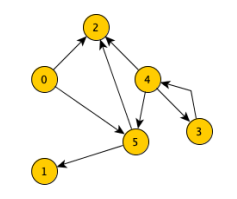
\includegraphics[width=5cm]{images/grafo-diretto.PNG}
    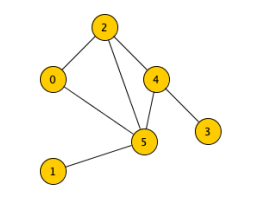
\includegraphics[width=5.2cm]{images/grafo-non-diretto.PNG}
    \caption{Grafo diretto e grafo non diretto}
    \label{fig:grafo-diretto-non}
\end{figure}

Un grafo di dice \textit{sparso} se il numero di archi è dello stesso ordine del numero dei nodi $m=O(n)$, oppure si dice \textit{denso} se il numero di archi è quadratico rispetto al numero di nodi $m=\Omega(n^2)$.
Ad esempio un grafo vuoto (senza archi) è sparso, mentre un grafo completo (con il massimo numero di archi) è denso. 
Inoltre un grafo non sparso non è necessariamente denso, ad esempio si possono avere $\Theta(n\log n)$ archi.

Un albero è un grafo sparso, connesso (partendo da qualunque nodo si possono raggiungere tutti gli altri) e senza cicli (aciclico).

\begin{Lemma}{Archi in un albero}{}
    Un albero ha sempre $m=n-1$ archi la cui prova è fornita per induzione sul numero $n$ di nodi.
    \begin{demonstration}\phantom{}
        \begin{itemize}
            \item Caso base: in un albero con $n=1$ nodi ci saranno $m=0$ archi;
            \item Ipotesi induttivo: assumiamo vero che in un albero con $n$ nodi ci sono $m=n-1$ archi;
            \item Passo induttivo: in un albero con $n+1$ nodi, tolgo una foglia e il rispettivo arco, mi rimane un albero aciclico con $n$ nodi che per ipotesi induttiva ha $m=n-1$ archi. Aggiungendo la foglia e l'arco eliminati precedentemente ottengo un albero con $n+1$ nodi e $m=n$ archi.
        \end{itemize}
    \end{demonstration}
\end{Lemma}

Un grafo \textit{planare} è un grafo sparso che può essere rappresentato su una superficie piana in modo che gli archi non si sovrappongano. Secondo il teorema di Eulero un grafo planare di $n\geq3$ nodi non ha al più di $3n-6$ archi, e se $n>3$ e non vi sono cicli di lunghezza 3, allora si hanno massimo $2n-4$ archi.

\section{Rappresentare un grafo}
I metodi che studieremo per rappresentare un grafo sono due: con matrice di adiacenza e con liste di adiacenza.
\begin{itemize}
    \item Il modo più semplice per rappresentare un grafo è con una matrice di adiacenza $nxn$ dove la cella \verb|M[i][j]| è 1 solo se c'è un arco diretto da $i$ a $j$. Nel caso di grafi non diretti questa matrice è simmetrica perché la cella \verb|M[i][j]| contiene lo stesso valore della cella \verb|M[j][i]|. Lo spazio richiesto per questa struttura è $O(n^2)$.
    \item Un altro modo di rappresentare un grafo è tramite le liste di adiacenza che utilizzano una lista di liste \verb|G|. La lista ha tanti elementi quanti sono i nodi del grafo e, \verb|G[x]| è a sua volta una lista contenente i nodi adiacenti al nodo $x$, vale a dire quelli da archi che partono da $x$.
\end{itemize}

Con questo secondo metodo è più efficiente memorizzare grafi sparsi e, in un grafo diretto, ogni arco occuperà soltanto una lista (nella lista da dove l'arco parte) $O(n+m)$, mentre nei grafi non diretti, ogni arco comparirà due volte nelle liste (in entrambe le liste dei nodi che sono collegati dall'arco) $O(n+2m)$.

\begin{figure}[ht]
    \centering
    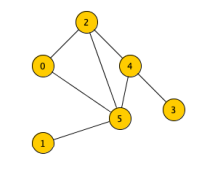
\includegraphics[height=3.5cm]{images/rapp-grafo1.PNG}
    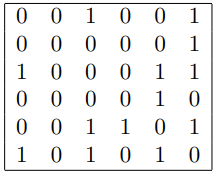
\includegraphics[height=3.5cm]{images/mat-bin1.PNG}
    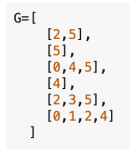
\includegraphics[height=3.5cm]{images/liste-adiac1.PNG}
    \caption{Rappresentazione di un grafo non diretto}
    \label{fig:rapp-grafo-nondiretto}
\end{figure}

\begin{figure}[ht]
    \centering
    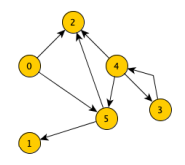
\includegraphics[height=3.5cm]{images/rapp-grafo2.PNG}
    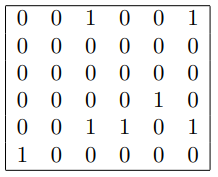
\includegraphics[height=3.5cm]{images/mat-bin2.PNG}
    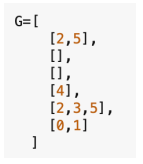
\includegraphics[height=3.5cm]{images/liste-adiac2.PNG}
    \caption{Rappresentazione di un grafo diretto}
    \label{fig:rapp-grafo-diretto}
\end{figure}

\begin{Lemma}{Nodi con lo stesso grado}{}
    In un grafo con $n\geq2$ nodi ci sono almeno due nodi che hanno lo stesso grado (stesso numero di archi che incidono sul nodo).

    \begin{demonstration}
        Assumiamo il grafo connesso. Se non lo fosse, prendiamo una componente connessa qualsiasi con almeno due nodi (se non c'è, ci sono almeno due nodi con grado 0). 
        
        Se $n$ è il numero dei nodi della componente connessa, i gradi sono nell'intervallo $[1, n - 1]$. Applicando il principio dei cassetti (o legge del buco della piccionaia)\footnote{Se $n+k$ oggetti sono messi in $n$ cassetti, allora almeno un cassetto deve contenere più di un oggetto.} si ha necessariamente che almeno due nodi devono avere lo stesso grado.
    \end{demonstration}
\end{Lemma}

\subsection{Ricerca di un pozzo}

In un grafo diretto un \textit{pozzo} è un nodo senza archi uscenti, mentre, è un \textit{pozzo universale} un pozzo verso cui gli altri nodi hanno un arco. In un grafo diretto possono essere presenti fino ad $n$ pozzi e il pozzo universale se c'è, è unico.

\begin{Algoritmo}{Verifica pozzo universale in $O(n^2)$}{}
    Un algoritmo di tempo $O(n^2)$ per verificare se un grafo diretto ha un pozzo universale, controlla in ogni nodo se la riga della matrice contiene tutti 0, ovvero se il nodo non ha archi uscenti, e se la colonna della matrice è formata da tutti 1 (tranne per l'elemento \verb|M[u][u]|), ovvero se il nodo ha solo archi entranti.
    
    \begin{minipage}[c]{0.45\textwidth}
    \begin{lstlisting}[language=Python]
    def pozzoU(u, M):
        if sum(M[u])!=0:
            return false
        for i in range(len(M)):
            if i!=u and M[i][u]!=1:
                return false
        return true

    def PU(M):
        for i in range(len(M)):
            if pozzoU(i, M):
                return ture
        return false
    \end{lstlisting}
    \end{minipage}
    \hspace{2cm}
    \begin{minipage}[c]{0.30\textwidth}
        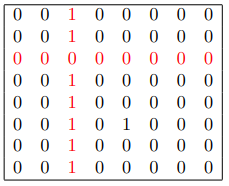
\includegraphics[width=1\textwidth]{images/esercizio-pozzo-univ1.PNG}
    \end{minipage}      
\end{Algoritmo}

\begin{Algoritmo}{Verifica pozzo universale in $\Theta(n)$}{}
    Un algoritmo di tempo $\Theta(n)$ per verificare se un grafo diretto ha un pozzo universale, utilizza una lista \verb|A| con tutti i nodi e li confronta tra di loro. Se il nodo \verb|a| ha un arco verso il nodo \verb|b|, \verb|a| viene eliminato dalla lista, altrimenti viene eliminato \verb|b|. Al termine di questo procedimento resta un unico nodo da controllare se è un pozzo universale.

    \begin{lstlisting}[language=Python]
    def PU1(M):
        A=[x for x in range(len(M))]
        while len(A)>1:
            a=A.pop()
            b=A.pop()
            if M[a][b]==1:
                A.append(b)
            else:
                A.append(a)
        a=A.pop()
        return pozzoU(a, M)
    \end{lstlisting}

    Ad ogni passo l'algoritmo elimina un nodo dalla lista $\Theta(n-1)$ e per verificare se un nodo è un pozzo universale impiega $O(n)$. Quindi la complessità totale è $\Theta(n)$.
\end{Algoritmo}


\section{Visite in profondità (DFS)}

\begin{Algoritmo}{Visita in profondità (DFS) tramite matrice e liste di adiacenza}{}
    \textit{Dato un grafo $G$ ed un suo nodo $u$ vogliamo sapere quali nodi del grafo sono raggiungibili a partire dal nodo $u$.}

    Per risolvere il problema visitiamo i nodi del grafo tramite la ricorsione, con l'aggiunta di una lista di nodi già visitati \verb|V| per non entrare in un loop del grafo. La corretta soluzione con la matrice di adiacenza è:

    \begin{lstlisting}[language=Python]
    def DFS(u, M):
        def DFSr(u, M, V):
            V[u]=1
            for i in range(len(M)):
                if M[u][i]==1 and V[i]==0:
                    DFSr(i, M, V)
        
        V=[0 for i in range(len(M))]
        DFSr(u, M, V)
        return V
    \end{lstlisting}

    La complessità di questo algoritmo è $O(n)\Theta(n)=O(n^2)$.

    Si può risolvere lo stesso problema anche con le liste di adiacenza:

    \begin{lstlisting}[language=Python]
    def DFS(u, G):
        def DFSr(u, G, V):
            V[u]=1
            for x in G[u]:
                if V[x]==0:
                    DFSr(x, G, V)
        
        V=[0 for i in G]
        DFSr(u, G, V)
        return V
    \end{lstlisting}

    La complessità di questo algoritmo è $O(n+m)$.
\end{Algoritmo}

\begin{Thm}{Correttezza dell'algoritmo di visita in profondità (DFS)}{}
    Dato un grafo $G$ ed un suo nodo $u$, l'algoritmo di visita in profondità (DFS) ci permette di conoscere quali nodi sono raggiungibili a partire dal nodo $u$, e questi nodi si troveranno nel vettore $V$ al termine dell'algoritmo con valore 1.
    \begin{demonstration}
        Supponiamo per assurdo che $x$ è un nodo raggiungibile ma alla fine dell'algoritmo abbiamo \verb|V[x]=0|. Tornando all'indietro sul percorso dei nodi, essendo \verb|V[x]=0| non è possibile arrivare al nodo di partenza $u$. Viceversa il nodo $x$ non è raggiungibile partendo dal nodo $u$ (contraddizione).
    \end{demonstration}
\end{Thm}

Con una visita DFS gli archi del grafo si bipartiscono in quelli che nel corso della visita sono stati attraversati (perché permettevano di raggiungere nuovi nodi) e gli altri. I nodi visitati e gli archi effettivamente attraversati formano un albero detto \textit{albero DFS}.

\begin{figure}[ht]
    \centering
    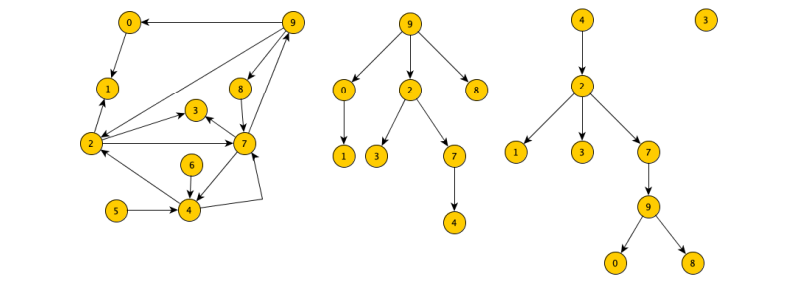
\includegraphics[width=1\textwidth]{images/alberi-DFS.PNG}
    \caption{Alberi DFS}
    \label{fig:alberi-dfs}
\end{figure}

\subsection{Vettore dei padri}

Un albero può essere memorizzato tramite il \textit{vettore dei padri}. Il vettore dei padri \verb|P| di un albero \verb|T| di $n$ nodi ha almeno $n$ componenti: se $i$ è un nodo dell'albero \verb|P[i]| contiene il padre del nodo $i$ (il padre della radice per convenzione è la radice stessa); se $i$ non è un nodo dell'albero \verb|P[i]| per convenzione contiene -1.

\begin{figure}[ht]
    \centering
    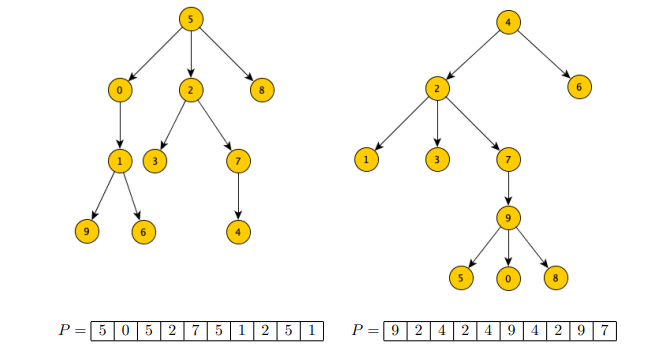
\includegraphics[width=0.8\textwidth]{images/vettore-padri.PNG}
    \caption{Vettore dei padri}
    \label{fig:vettore-padri}
\end{figure}

\begin{Algoritmo}{Visita in profondità (DFS) per il vettore dei padri}{}
    Modificando lievemente la procedura DFS è possibile fare in modo che restituisca il vettore dei padri \verb|P| anziché il vettore dei visitati.

    \begin{lstlisting}[language=Python]
    def Padri(u, G):
        def DFSr(u, G, P):
            for x in G[u]:
                if P[x]==-1:
                    P[x]=u
                    DFSr(x, G, P)
        
        P=[-1]*len(G)
        P[u]=u
        DFSr(u, G, P)
        return P
    \end{lstlisting}

    Al termine \verb|P[v]| contiene -1 se $v$ non è stato visitato altrimenti contiene il padre di $v$ nell'albero DFS.
\end{Algoritmo}

Spesso non ci basta sapere se un nodo $y$ è raggiungibile a partire dal nodo $x$ del grafo: nel caso la risposta sia positiva vogliamo anche un cammino che ci permetta di andare da $x$ a $y$.

\begin{Algoritmo}{Cammino con il vettore dei padri}{}
    Il vettore dei padri dell'albero DFS radicato in $x$ permette di ricavare facilmente il cammino per $y$: basta controllare che il nodo $y$ sia nell'albero e poi da $y$ risalire alla radice ed effettuare il “reverse” dei nodi incontrati.

    Questo problema può essere risolto in tempo $O(n)$ con un approccio iterativo o ricorsivo:

    \begin{minipage}[t]{0.50\textwidth}
    \begin{lstlisting}[language=Python]
    def Cammino(u, P):
        if P[u]==-1:
            return []
        path = []
        while P[u]!=u:
            path.append(u)
            u=P[u]
        path.append(u)
        path.reverse()
        return path
    \end{lstlisting}
    \end{minipage}
    \hspace{-1cm}
    \begin{minipage}[t]{0.50\textwidth}
    \begin{lstlisting}[language=Python]
    def Cammino(u, P):
        if P[u]==-1:
            return []
        if P[u]==u:
            return [u]
        return Cammino(P[u], P)+[u]
    \end{lstlisting}
    \end{minipage}
\end{Algoritmo}

Se esistono più cammini che dal nodo $x$ portano al nodo $y$ la procedura appena vista non garantisce di restituire il cammino minimo.

\subsection{Colorazione dei grafi}
Dato un grafo connesso $G$ ed un intero $k$ vogliamo sapere se è possibile colorare i nodi del grafo in modo che nodi adiacenti abbiamo sempre colori distinti.

\begin{figure}[ht]
    \centering
    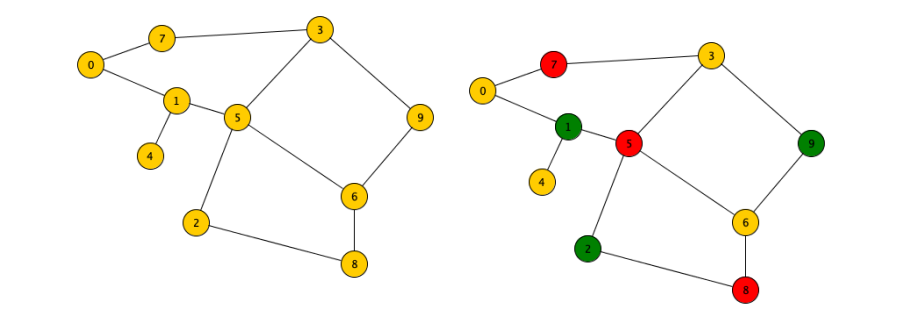
\includegraphics[width=1\textwidth]{images/grafo-3colorabile.PNG}
    \caption{Esempio di grafo 3-colorabile}
    \label{fig:grafo-3colorabile}
\end{figure}

\begin{Thm}{Teorema dei quattro colori}{}
    Secondo il teorema dei 4 colori: un grafo planare richiede al più 4 colori per essere colorato.
\end{Thm}

In generale un grafo può richiedere anche $\Theta(n)$ colori. Non è noto nessun algoritmo polinomiale che, dato un grafo planare $G$, determini se $G$ è 3-colorabile. 

\begin{Lemma}{Grafo 2-colorabile}{}
    Un grafo è 2-colorabile se e solo se non contiene cicli di lunghezza dispari.
    \begin{demonstration}
        Un ciclo di lunghezza dispari rende impossibile la colorazione del grafo con due colori.
        
        \begin{minipage}{\textwidth}
            \centering
            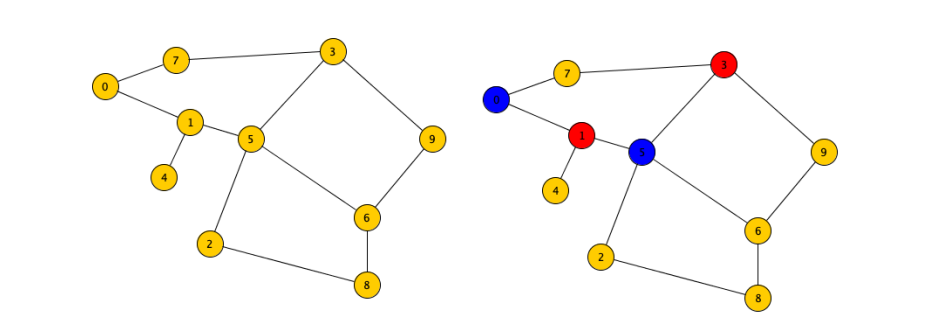
\includegraphics[width=0.9\linewidth]{images/grafo-2colorabile.PNG}
            %\captionof{figure}{Esempio}
        \end{minipage}
        L'algoritmo di bi-colorazione che segue prova che un grafo senza cicli dispari può sempre essere 2-colorato.
        \end{demonstration}
\end{Lemma}

\begin{Algoritmo}{Algoritmo di bi-colorazione}{}
    L'algoritmo opera nel seguente modo:
    \begin{enumerate}
            \item Colora il nodo 0 col colore 0.
            \item Effettua una visita in profondità del grafo a partire dal nodo 0. Nel corso della visita, a ciascun nodo $x$ che incontri assegna uno dei due colori 0 e 1. Scegli il colore da assegnare in modo che sia diverso dal colore assegnato al nodo padre che ti ha portato a visitare $x$.
        \end{enumerate}
        \begin{lstlisting}[language=Python]
    def colora(G):
        def DFSr(x, G, colore, c):
            colore[x]=c
            for y in G[x]:
                if colore[y]==-1:
                    DFSr(y, G, colore, 1-c)
        
        colore=[-1 for v in G]
        DFSr(0, G, colore, 0)
        return colore
        \end{lstlisting}

        La complessità dell'algoritmo è quella di una semplice visita del grafo connesso da colorare: $O(n+m)=O(m)$ (dipende dal fatto che in un grafo connesso $m\geq n-1$).
\end{Algoritmo}

\begin{Thm}{Correttezza dell'algoritmo di bi-colorazione}{}
    Siano $x$ e $y$ due nodi adiacenti in G, consideriamo i due possibili casi e facciamo vedere che in entrambi i casi i due nodi al termine avranno colori opposti.

    \begin{demonstration}\phantom{}
    \begin{enumerate}
        \item L'arco $(x, y)$ viene attraversato durante la visita. In questo caso banalmente i due nodi hanno colori distinti.
        \item L'arco $(x, y)$ non viene attraversato durante la visita. Sia $x$ il nodo visitato prima. Esiste un cammino in $G$ che da $x$ porta a $y$ (quello seguito dalla visita), questo cammino si chiude a formare un ciclo con l'arco $(y, x)$. Il ciclo è di lunghezza pari per ipotesi, quindi il cammino è di lunghezza dispari. Poiché sul cammino i colori si alternano il primo nodo $(x)$ e l'ultimo nodo $(y)$ del cammino avranno colori diversi. 
    \end{enumerate}    
    \end{demonstration}
    
\end{Thm}

\subsection{Componenti connesse}
Una \textit{componente connessa} di un grafo non diretto è un sotto-grafo composto da un insieme massimale di nodi connessi da cammini. Un grafo si dice connesso se ha una sola componente connessa.

\begin{figure}[ht]
    \centering
    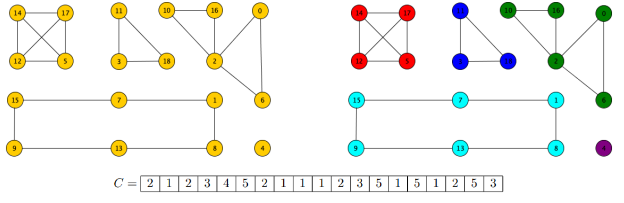
\includegraphics[width=1\textwidth]{images/componenti-connesse.PNG}
    \caption{Esempio di grafo con componenti connesse}
    \label{fig:componenti-connesse}
\end{figure}

Vogliamo calcolare il vettore $C$ delle componenti connesse di un grafo $G$. Vale a dire il vettore $C$ che ha tanti elementi quanti sono i nodi del grafo e $C[u]=C[v]$ se e solo se $u$ e $v$ sono nella stessa componente connessa.

\begin{Algoritmo}{Algoritmo di ricerca delle componenti connesse}{}
    \textit{Il seguente algoritmo calcola il vettore $C$ delle componenti connesse di un grafo $G$.}
\begin{lstlisting}[language=Python]
    def Componenti(G):
        def DFSr(x, G, C, c):
            C[x]=c
            for y in G[x]:
                if C[y]==0:
                    DFSr(y, G, C, c)
        
        C=[0]*len(G)
        c=0
        for x in range(len(G)):
            if C[x]==0:
                c+=1
                DFSr(x, G, C, c)
        return C
\end{lstlisting}
    La complessità della procedura è $O(n + m)$.
\end{Algoritmo}

\subsubsection*{Componenti fortemente connesse}
Una \textit{componente fortemente connessa} di un grafo diretto è un sotto-grafo composto da un insieme massimale di nodi connessi da cammini, ovvero se da un nodo posso arrivare a tutti gli altri e da tutti gli altri posso arrivare a quel nodo. Un grafo diretto si dice fortemente connesso se ha una sola componente. 

\begin{figure}[ht]
    \centering
    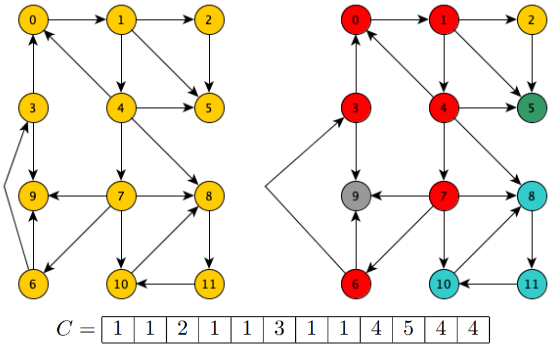
\includegraphics[width=0.6\textwidth]{images/fortemente-connesse.PNG}
    \caption{Esempio di grafo con componenti fortemente connesse}
    \label{fig:fortemente-connesse}
\end{figure}

Vogliamo calcolare il vettore $C$ delle componenti fortemente connesse di un grafo $G$. Vale a dire il vettore $C$ che ha tanti elementi quanti sono i nodi del grafo e $C[u]=C[v]$ se e solo se $u$ e $v$ sono nella stessa componente fortemente connessa.

L'algoritmo utilizzato per le componenti connesse non funziona nel caso di componenti fortemente connesse. Il problema risiede nel fatto che se c'è un cammino che da $x$ mi porta a $y$ questo non implica che $x$ e $y$ sono nella stessa componente fortemente connessa, perché questo sia vero è necessario che ci sia anche un cammino che da $y$ mi porti a $x$.

Dato un grafo diretto $G$ il \textit{grafo trasposto} (o complementare) di $G$ ($G^C = (V, E^C)$) ha gli stessi nodi di $G$ ma archi con direzione opposta.

\begin{figure}[ht]
    \centering
    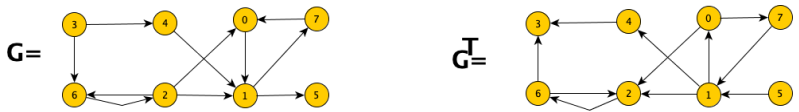
\includegraphics[width=0.9\textwidth]{images/grafo-trasposto.PNG}
    \caption{Esempio di grafo trasposto}
    \label{fig:grafo-trasposto}
\end{figure}

\begin{Lemma}{Grafo complementare connesso}{}
    Almeno uno tra $G$ e $G^C$ è connesso.  
    \begin{demonstration}
        Consideriamo il caso in cui $G$ non sia connesso (altrimenti non c'è nulla da dimostrare perché $G$ è connesso). Siano $u$, $v$ due nodi qualsiasi di $G$. Se $u$ e $v$ appartengono a due diverse componenti connesse di $G$, allora c'è l'arco $(u, v)$ in $G^C$. Se sono nella stessa componente connessa diciamo $G_1$, prendiamo un nodo qualsiasi $z$ in un'altra componente connessa $G_2$. Gli archi $(u, z)$ e $(z, v)$ sono allora in $G^C$ e quindi c'è il cammino $u$ $z$ $v$ in $G^C$.
    \end{demonstration}
    
\end{Lemma}

\begin{Algoritmo}{Algoritmo di ricerca delle componenti fortemente connesse}{}
    \textit{Dato il grafo diretto $G$ ed un suo nodo $u$, l'algoritmo restituisce i nodi della componente fortemente connessa che contiene $u$ in tre passi:}
    \begin{enumerate}
        \item calcola l'insieme $A$ dei nodi di $G$ raggiungibili da $u$ ($O(n+m)$), effettuando una visita sul nodo e ottenendo il vettore dei visitati;
        \item calcola l'insieme $B$ dei nodi di $G$ che portano a $u$. Per eseguire efficientemente questo passo si può ricorrere al grafo trasposto di $G$ ($O(n+m)$);
        \begin{lstlisting}[language=Python]
    def Trasposto(G):
        GT=[[] for _ in G]
        for i in range(len(G)):
            for v in G[i]
                GT[v].append(i)
        return GT
        \end{lstlisting}
        \item restituisci l'intersezione dei due insiemi $A$ e $B$ ($O(n)$).
        \begin{lstlisting}[language=Python]
    def Intersezione(V1, V2):
        V=[0]*len(V1)
        for i in range(len(V1)):
            if V1[i]==V2[i]==1:
                V[i]=1
        return V
        \end{lstlisting}
    \end{enumerate}

L'algoritmo risultante è il seguente:
 \begin{lstlisting}[language=Python]
    def ComponenteFC(x, G):
        visitati1=DFS(x, G)
        G1=Trasposto(G)
        visitati2=DFS(x, G1)
        return Intersezione(visitati1, visitati2)
\end{lstlisting}
    La sua complessità è data dalla somma dei tre passi:
    \begin{equation*}
        O(n+m)+O(n+m)+O(n+m)+O(n)=O(n+m)
    \end{equation*}
\end{Algoritmo}

Utilizzando l'algoritmo \verb|ComponenteFC(x, G)| come subroutine posso ottenere un algoritmo per calcolare il vettore CF delle componenti fortemente connesse:
\begin{lstlisting}[language=Python]
    def compFC(G):
        FC=[0]*len(G)
        c=0
        for i in range(len(G)):
            if FC[i]==0:
                E=ComponenteFC(i, G)
                c+=1
                for x in E:
                    FC[x]=c
        return FC
\end{lstlisting}

La complessità dell'algoritmo è $\Theta(n) * O(n + m) = O(n^2 + nm) = O(n^3)$.

Per il calcolo del vettore CF delle componenti fortemente connesse sono noti diversi algoritmi non banali che lavorano in tempo $O(n+m)$ (ad esempio l'algoritmo di Tarjan o quello di Kosaraju).

\subsection{Ordinamento topologico}
Spesso un grafo diretto cattura relazioni di propedeuticità (un arco da $a$ a $b$ indica che $a$ è propedeutico a $b$). Potrò rispettare tutte le propedeuticità se riesco ad ordinare i nodi del grafo in modo che gli archi (le frecce) vadano tutti da sinistra verso destra. Questa ordinamento è detto \textit{ordinamento topologico}.

\begin{figure}[ht]
    \centering
    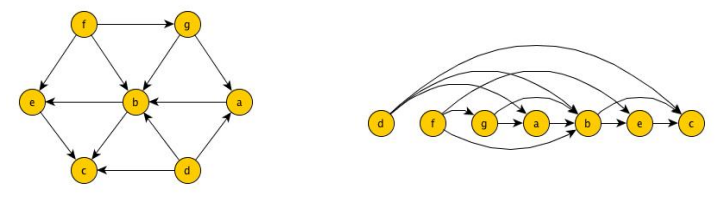
\includegraphics[width=0.9\textwidth]{images/ordinamento-topologico.PNG}
    \caption{Esempio di ordinamento topologico}
    \label{fig:ordinamento-topologico}
\end{figure}

Un grafo diretto può avere da $0$ ad $n!$ ordinamenti topologici. Perché $G$ possa avere un ordinamento topologico è necessario che sia un \textit{DAG} (ovvero un grafo diretto aciclico). La presenza di un ciclo nel grafo implica che nessuno dei nodi del ciclo possa comparire nell'ordine giusto. Un DAG ha sempre un nodo sorgente (un nodo in cui non entrano archi).

\begin{Algoritmo}{Algoritmo di ordinamento topologico}{}
    Posso costruire l'ordinamento topologico dei nodi del DAG in questo modo:
    \begin{enumerate}
        \item Inizio la sequenza dei nodi con una sorgente;
        \item Cancello dal DAG quel nodo sorgente e le frecce che partono da lui. Ottengo un nuovo DAG;
        \item Itero questo ragionamento finché non ho sistemato in ordine lineare tutti i nodi. 
    \end{enumerate}

    \begin{lstlisting}[language=Python]
    def SortTop(G):
        gradoEnt=[0]*len(G)
        for i in range(len(G)):
            for j in G[i]:
                gradoEnt[j]+=1
        sorgenti=[]
        for i in range(len(G)):
            if gradoEnt[i]==0:
                sorgenti.append(i)
        ST=[]
        while len(sorgenti)>0:
            x=sorgenti.pop()
            ST.append(x)
            for y in G[x]:
                gradoEnt[y]-=1
                if gradoEnt[y]==0:
                    sorgenti.append(y)
        if len(ST)==len(G):
            return ST
        return []
    \end{lstlisting}
    Inizializzare il vettore dei gradi entranti costa $O(n + m)$, inizializzare l'insieme delle sorgenti costa $O(n)$, il while viene iterato $O(n)$ volte e il costo totale del for al termine del while è $O(m)$. Il costo dell'algoritmo è $O(n + m)$.
\end{Algoritmo}

\begin{Algoritmo}{Algoritmo alternativo di ordinamento topologico con DFS}{}
    Posso costruire un algoritmo alternativo basato sulla visita DFS per l'ordinamento topologico dei nodi del DAG in questo modo:
    \begin{enumerate}
        \item Effettua una visita del DAG a partire dal nodo 0;
        \item Man mano che termina la visita dei vari nodi, inseriscili in una lista;
        \item Restituisci come ordinamento dei nodi il reverse della lista.
    \end{enumerate}

    \begin{lstlisting}[language=Python]
    def SortT(G):
        def DFSr(x, G, visitati, lista):
            visitati[x]=1
            for y in G[x]:
                if visitati[y]==0:
                    DFSr(y, G, visitati, lista)
            lista.append(x)

        visitati=[0 for _ in G]
        lista=[]
        for x in range(len(G)):
            if vistati[x]==0:
                DFSr(x, G, visitati, lista)
        lista.reverse()
        return lista
    \end{lstlisting}
    La complessità è $O(n+m)+O(n)=O(n+m)$.
\end{Algoritmo}

\begin{Thm}{Correttezza dell'algoritmo alternativo di ordinamento topologico con DFS}{}
    Siano $x$ e $y$ due nodi in $G$, con arco che va da $x$ a $y$. In entrambi i casi nella lista, prima di effettuare il reverse, $y$ precede $x$. 
    \begin{demonstration}
        Se l'arco $(x, y)$ viene attraversato durante la visita. In questo caso banalmente la visita di $y$ finisce prima della visita di $x$ e $y$ finisce nella lista prima che ci finisca $x$.

        Se l'arco $(x, y)$ non viene attraversato durante la visita. Durante la visita di $x$ il nodo $y$ è già stato visitato e la sua visita è anche gia terminata (infatti da $y$ non c'è un cammino che porta a $x$, in caso contrario nel DAG ci sarebbe un ciclo), anche in questo caso $y$ finisce nella lista prima che ci finisca $x$.
    \end{demonstration}
\end{Thm}

\subsection{Ricerca dei cicli}
Dato un grafo $G$ (diretto o non diretto) ed un suo nodo $u$ vogliamo sapere se da $u$ è possibile raggiungere un ciclo in $G$.

\begin{Algoritmo}{Algoritmo sbagliato per i cicli}{}
    L'idea di partenza (sbagliata) è: visita il grafo, e se nel corso della visita incontri un nodo già visitato interrompila e restituisci \verb|True|, se al contrario la visita termina regolarmente restituisci \verb|False|.
    
    \begin{lstlisting}[language=Python]
    def ciclo(u, G):
        def DFSr(u, G, visitati):
            visitati[u]=1
            for v in G[u]:
                if visitati[v]==1:
                    return True
                if DFSr(v, G, visitati):
                    return True
            return False
    
        visitati=[0]*len(G)
        return DFSr(u, G, visitati)
    \end{lstlisting}

    Il codice è sbagliato sia con grafi non diretti che con grafi diretti:
    \begin{itemize}
        \item Il codice è sbagliato perché (per come è codificato il grafo non diretto) se $x$ ha un arco che lo collega a $y$ nella lista di adiacenza di $x$ è presente $y$ e nella lista di adiacenza di $y$ è presente $x$. Questo viene interpretato erroneamente come un ciclo di lunghezza 2 e la procedura proposta termina quindi sempre con \verb|True|.
        \item Il codice è sbagliato perché incontrare in un grafo diretto un nodo già visitato non significa necessariamente che si è in presenza di un ciclo e la procedura può terminare con \verb|True| anche in assenza di ciclo.
    \end{itemize}

    \begin{minipage}{\textwidth}
        \centering
        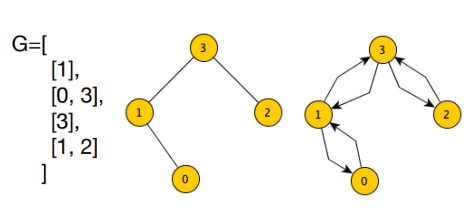
\includegraphics[width=0.45\linewidth]{images/cicli-sbagliato.PNG}
        \hspace{1cm}
        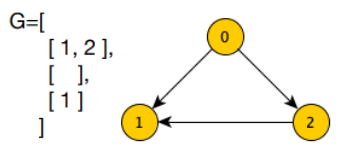
\includegraphics[width=0.30\linewidth]{images/cicli-sbagliato2.PNG}
        \captionof{figure}{Cicli sbagliati di grafi non diretti e diretti}
    \end{minipage}
\end{Algoritmo}

\begin{Algoritmo}{Algoritmo per i cicli con i grafi non diretti}{}
   Per risolvere il problema, durante la visita alla ricerca del ciclo, devo distinguere nella lista di adiacenza di ciascun nodo $y$ che incontro il nodo $x$ che mi ha portato a visitarlo (il padre di $y$ nell'albero DFS).
    
    \begin{lstlisting}[language=Python]
    def ciclo(u, G):
        def DFSr(u, padre, G, visitati):
            visitati[u]=1
            for v in G[u]:
                if visitati[v]==1:
                    if v!=padre:
                        return True
                else:
                    if DFSr(v, u, G, visitati):
                        return True
            return False
    
        visitati=[0]*len(G)
        return DFSr(u, u, G, visitati)
    \end{lstlisting}

    La complessità $O(n)$ è dovuta al fatto che se il grafo non contiene cicli allora ha al più $n-1$ archi e quindi $O(n+m)=O(n)$. Se al contrario il grafo contiene cicli se ne trova uno dopo aver considerato al più $n$ archi e a quel punto la procedura termina la visita.
\end{Algoritmo}

\begin{Algoritmo}{Algoritmo per i cicli con i grafi diretti}{}
    Durante la visita DFS posso incontrare nodi già visitati in tre modi diversi: archi in avanti (cioè le frecce dirette da un antenato a un discendente), archi all'indietro (cioè le frecce dirette da un discendente ad un antenato) e archi di attraversamento. Solo la presenza di archi all'indietro testimonia la presenza di un ciclo.

    Per risolvere il problema, durante la visita DFS alla ricerca del ciclo, devo poter distinguere la scoperta di nodi già visitati grazie ad un arco all'indietro dagli altri. Posso individuare i visitati da archi all'indietro notando che solo nel caso di archi all'indietro la visita del nodo già visitato ha terminato la sua ricorsione.

    Per il vettore $V$ dei visitati uso tre step:
    \begin{itemize}
        \item in $V$ un nodo vale 0 se il nodo non è stato ancora visitato;
        \item in $V$ un nodo vale 1 se il nodo è stato visitato ma la ricorsione su quel nodo non è ancora finita;
        \item in $V$ un nodo vale 2 se il nodo è stato visitato e la ricorsione su quel nodo è finita.
    \end{itemize}

    In questo modo scopro un ciclo quando trovo un arco diretto verso un nodo già visitato che si trova nello stato 1.

    \begin{lstlisting}[language=Python]
    def ciclo(u, G):
        def DFSr(u, G, visitati):
            visitati[u]=1
            for v in G[u]:
                if visitati[v]==1:
                    return True
                if visitati[v]==0:
                    if DFSr(v, G, visitati):
                        return True
            visitati[u]=2
            return False
            
        visitati=[0]*len(G)
        return DFSr(u, G, visitati)
    \end{lstlisting}

    La complessità è $O(n+m)$.
\end{Algoritmo}

Se voglio sapere se un grafo (diretto o non diretto) contiene un ciclo o meno, devo visitarlo tutto non importa il punto da cui parto. Non è difficile modificare le procedure appena viste senza alterarne la complessità $O(n+m)$.

\subsection{Ricerca dei ponti}
In un grafo la connessione è una proprietà che può andar persa con la perdita di un arco.
Un arco la cui eliminazione disconnette il grafo è detto \textit{ponte}. I ponti rappresentano criticità del grafo ed è quindi utile identificarli. Il grafo può non avere neanche un ponte così come avere tutti i suoi archi come ponti.

\begin{figure}[ht]
    \centering
    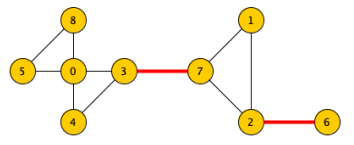
\includegraphics[width=7cm]{images/ponte.PNG}
    \caption{Esempio di ponte}
    \label{fig:ponte}
\end{figure}

\begin{Lemma}{Ponte in un grafo}{}
    \begin{minipage}[c]{0.65\textwidth}
    Sia $\{u, v\}$ un arco dell'albero DFS con u padre di $v$. L'arco $\{u, v\}$ è un ponte se e solo se non ci sono archi tra i nodi del sottoalbero radicato in $v$ e il nodo $u$ o nodi antenati di $u$.
    \begin{demonstration}
    Sia $\{x, y\}$ un arco tra un antenato di $u$ e un discendente di $v$. Dopo l'eliminazione dell'arco $\{u, v\}$ tutti i nodi dell'albero restano comunque connessi grazie all'arco $\{x, y\}$.

    Se, al contrario $\{x, y\}$ non è un arco tra un antenato di $u$ e un discendente di $v$, l'eliminazione dell'arco $\{u, v\}$ disconnette i nodi dell'albero radicato in $v$ dal resto del grafo.
    \end{demonstration}
    \end{minipage}
    \hfill
    \begin{minipage}[c]{0.30\textwidth}
        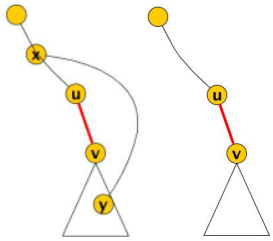
\includegraphics[width=1\textwidth]{images/ponte2.PNG}
    \end{minipage}

    \begin{osservation}
        Nel momento in cui l'arco $\{u, v\}$ viene attraversato per raggiungere il nodo $v$ da visitare, il nodo $u$ non ha informazioni per decidere se dal sotto-albero radicato in $v$ partono archi verso suoi antenati (quindi scoprire se $\{u, v\}$ è ponte o meno). Ma gli sarà possibile scoprirlo al termine della visita di $v$ se riceve da $v$ la giusta informazione.    
    \end{osservation}
\end{Lemma}

\begin{Algoritmo}{Ricerca dei ponti in un grafo}{}
    \textit{Dato un grafo connesso $G$ determinare l'insieme di ponti del grafo.}

    \begin{itemize}
        \item Una prima soluzione basata sulla ricerca esaustiva: prova per ogni arco del grafo se questo è ponte o meno. Verificare se un arco $\{a, b\}$ è un ponte per $G$ richiede tempo $O(m)$. Basta ad esempio eliminare l'arco $\{a, b\}$ da $G$ e, con una visita DFS, controllare se $b$ è raggiungibile a partire da $a$. La complessità di questo algoritmo è $m * O(m) = O(m^2) = O(n^4)$.
        \item Vedremo ora che il problema è risolvibile in tempo lineare nella dimensione del grafo $O(m)$. I ponti vanno ricercati unicamente tra gli $n-1$ archi dell'albero DFS. Infatti un arco non presente nell'albero DFS non può essere ponte (se lo elimino gli archi dell'albero DFS continuano a garantire la connessione).

        Durante la visita ogni nodo $x$ calcola la sua altezza nell'albero DFS e a fine visita restituisce l'altezza minima raggiungibile da nodi del sottoalbero radicato in $x$ tramite gli archi non presenti nell'albero DFS. Se non ci sono archi di questo tipo allora viene  restituito $+\infty$. Il nodo $u$ confrontando la sua altezza con il valore che gli viene segnalato dai figlio $v$ è in grado di decidere se l'arco $\{u, v\}$ è ponte o meno. $\{u, v\}$ è ponte se e solo se l'altezza di $u$ è strettamente minore del valore restituito da $v$.
        
        \begin{minipage}{\textwidth}
            \centering
            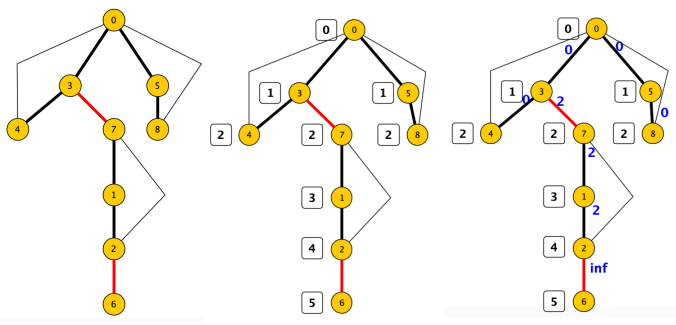
\includegraphics[width=0.8\textwidth]{images/ponte3.PNG}
        \end{minipage}

    L'algoritmo che risolve il problema con complessità $O(n+m)$ è il seguente:
    \begin{lstlisting}[language=Python]
    def TrovaPonti(G):
        def DFSModificata(x, t, G, Altezza, Ponti):
            from math import inf
            Altezza[x]=t
            ret=inf
            for y in G[x]:
                if Altezza[y]==-1:
                    a=DFSModificata(y, t+1, G, Altezza, Ponti)
                    if t<a:
                        Ponti.append((x, y))
                    ret=min(ret, a)
                elif Altezza[y]!=t-1:
                    ret=min(ret, Altezza[y])
            return ret
    
        Altezza=[-1]*len(G)
        Ponti=[]
        DFSModificata(0, 0, G, Altezza, Ponti)
        return Ponti
    \end{lstlisting}
    \end{itemize}
\end{Algoritmo}

\section{Visita in ampiezza (BFS)}
Dati due nodi $a$ e $b$ di un grafo $G$, definiamo distanza (minima) in $G$ di $a$ da $b$ il numero minimo di archi che bisogna attraversare per raggiungere $b$ a partire da $a$. La distanza è posta a $+\infty$ se $b$ non è raggiungibile partendo da $a$.

La visita in ampiezza (Breadth First Search) esplora i nodi del grafo partendo da quelli a distanza 1 dalla sorgente s. Poi visita quelli a distanza 2 e così via. L'algoritmo visita tutti i vertici a livello k prima di passare a quelli a livello k+1. Si genera un albero detto albero BFS dove si visitano nodi sempre più distanti dalla radice.

\begin{figure}[ht]
    \centering
    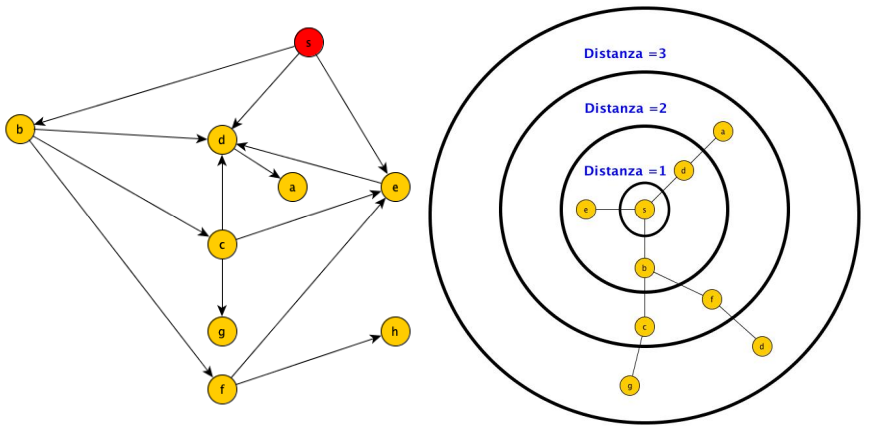
\includegraphics[width=0.8\linewidth]{images/BFS.PNG}
    \caption{Esempio di visita in ampiezza (BFS)}
    \label{fig:bfs}
\end{figure}

\begin{Algoritmo}{Visita in ampiezza (BFS)}{}
    \textit{Dato un grafo $G$ ed un suo nodo $x$ vogliamo conoscere le distanze di tutti i nodi di $G$ da $x$. Più precisamente vogliamo calcolare il vettore delle distanze $D$, dove in $D[y]$ troviamo la distanza di $y$ da $x$.}

    Per effettuare questo tipo di visita manteniamo in una coda i nodi visitati i cui adiacenti non sono stati ancora esaminati. Ad ogni passo, preleviamo il primo nodo dalla coda, esaminiamo i suoi adiacenti e se scopriamo un nuovo nodo lo visitiamo e lo aggiungiamo alla coda.

    \begin{lstlisting}[language=Python]
    def BFS(x, G):
        visitati=[0]*len(G)
        visitati[x]=1
        coda=[x]
        while coda:
            x=coda.pop(0)
            for y in G[u]:
                if visitati[y]==0:
                    visitati[y]=1
                    coda.append(y)
        return visitati
    \end{lstlisting}

    Un nodo finisce in coda al più una volta (poi risulterà visitato e non ci finisce più) quindi il while verrà eseguito $O(n)$ volte. Le liste di adiacenza dei nodi verranno scorse al più una volta quindi il costo totale dei \verb|for y in G[u]| sarà $0(m)$. Se le operazione di inserimento e cancellazione dalla coda richiedessero tempo $\Theta(1)$ avremmo complessità $O(n + m)$. Ma abbiamo implementato la coda tramite lista inserendo in coda e cancellando in testa, dove ogni inserimento in coda \verb|append()| costa $0(1)$, ogni estrazione in testa \verb|pop(0)| ha un costo proporzionale al numero di elementi presenti in quel momento nella coda/lista e questi elementi possono essere anche $O(n)$. Quindi il costo di questa implementazione dell'algoritmo è $O(n^2)$.

    L'implementazione alternativa di costo $O(n+m)$ consiste di effettuare solo cancellazioni logiche e non effettive: usando un puntatore che indica l'inizio della coda all'interno della lista, il puntatore si incrementa ogni volta che si cancella dalla coda. Alternativamente si può utilizzare la struttura dati \verb|deque| dal modulo \verb|collection| che permette di effettuare inserimenti e cancellazioni da entrambi i lati di una lista in tempo $O(1)$. In particolare può estrarre a sinistra \verb|popleft()| e inserire a sinistra \verb|appendleft()|.

    \begin{minipage}[t]{0.50\textwidth}
    \begin{lstlisting}[language=Python]
    def BFS(x, G):
        visitati=[0]*len(G)
        visitati[x]=1
        coda=[x]
        i=0
        while len(coda)>i:
            u=coda[i]
            i+=1
            for y in G[u]:
                if visitati[y]==0:
                    visitati[y]=1
                    coda.append(y)
        return visitati
    \end{lstlisting}
    \end{minipage}
    \hspace{-1cm}
    \begin{minipage}[t]{0.50\textwidth}
    \begin{lstlisting}[language=Python]
    def BFS(x, G):
        visitati=[0]*len(G)
        visitati[x]=1
        from collections import deque
        coda=deque([x])
        while coda:
            u=coda.popleft()
            for y in G[u]:
                if visitati[y]==0:
                    visitati[y]=1
                    coda.append(y)
        return visitati
    \end{lstlisting}
    \end{minipage}
\end{Algoritmo}

\begin{Thm}{Correttezza dell'algoritmo di visita in ampiezza (BFS)}{}
    Alla fine dell'algoritmo $visitati[u]$ contiene 1 se il nodo $u$ è raggiungibile da $x$, 0 altrimenti.
    \begin{demonstration}\phantom{}
    \begin{itemize}
        \item Se $u$ è raggiungibile a partire da $x$ allora \verb|visitati[u]=1|. Se $u$ è raggiungibile c'è un cammino $P$ da $x$ a $u$. Supponiamo per assurdo che al termine \verb|visitati[u]=0|. Sia $b$ il primo nodo che incontro nel cammino $P$ con \verb|v[b]=0| e a il suo predecessore (questi due nodi esistono perché il cammino comincia con $x$ e \verb|visitati[x]=1| e termina con $u$ e \verb|visitati[u]=0|). Un nodo che diventa 1 finisce in coda, quindi $a$ è finito in coda, ma l'algoritmo si ferma quando la coda si svuota quindi c'è stato un momento in cui $a$ è stato estratto dalla coda, in quel momento tutti i suoi vicini sono stati controllati e se non visitati sono stati visitati (e poi inseriti in coda) quindi anche $b$ è stato controllato e se non ancora visitato sarebbe stato visitato e posto a 1.
        \item Se $u$ non è raggiungibile a partire da $x$ allora \verb|visitati[u]=0|. Supponiamo per assurdo che al termine \verb|visitati[u]=1|. \verb|visitati[u]| diventa 1 quando viene inserito in coda ma questo accade perché risulta adiacente ad un nodo che viene estratto dalla coda, andando all'indietro questo processo deve terminare perché ciascun nodo viene inserito al più una volta nella coda quindi si crea un cammino da $x$ a $u$ il che è assurdo avendo supposto che $u$ non è raggiungibile da $x$.
    \end{itemize}
    \end{demonstration}
\end{Thm}

\begin{Algoritmo}{Vettore dei padri in BFS}{}
    Modifichiamo la procedura in modo che restituisca in $O(n+m)$ l'albero di visita BFS rappresentato tramite il vettore dei padri. 

    \begin{lstlisting}[language=Python]
    def BFSpadri(x, G):
        P=[-1]*len(G)
        P[x]=x
        coda=[x]
        i=0
        while len(coda)>i:
            u=coda[i]
            i+=1
            for y in G[u]:
                if P[y]==-1:
                    P[y]=u
                    coda.append(y)
        return P
    \end{lstlisting}

    Grazie al vettore dei padri $P$ in $O(n)$ potremo ottenere un cammino in $G$ dalla radice dell'albero al nodo $x$ (posto che  sia raggiungibile).
\end{Algoritmo}

\begin{Lemma}{Profondità minima nell'albero BFS}{}
    La distanza minima di un vertice $x$ da $s$ nel grafo $G$ equivale alla profondità di $x$ nell'albero BFS.
    \begin{demonstration}
    Si può dimostrare per induzione sulla distanza $d$ di $x$ da $s$. E' ovviamente vero per $d = 0$ in quanto l'unico vertice a distanza 0 da $s$ è $s$ stesso che è a profondità 0 nell'albero. Supponiamo sia vero per tutti i vertici con distanza al più $d-1$ e consideriamo quindi un vertice $x$ a distanza $d$. Sia $P$ un cammino minimo da $s$ a $x$ e sia $v$ il predecessore di $x$ in questo cammino. Per ipotesi induttiva è a profondità $d-1$ nell'albero e BFS. Se $x$ è stato inserito nell'albero grazie a $v$ allora si troverà a profondità $d$, assumiamo quindi che sia stato inserito nell'albero grazie ad un nodo $u\neq v$.

    La profondità di $u$ non può essere inferiore a $d-1$ altrimenti avremmo trovato un cammino che parte da $s$ e porta a $v$ (tramite $u$) di lunghezza inferiore a $d$. D'altra parte non può essere la profondità di $u$ maggiore di $d-1$ perché il nodo $v$ sarebbe stato visitato prima di $u$ e $x$ sarebbe stato inserito grazie al nodo $v$. Si deve necessariamente avere che la profondità di $u$ è $d-1$ e quindi la profondità di $v$ è comunque $d$.
    \end{demonstration}
    
    Grazie alla proprietà appena dimostrata i cammini prodotti grazie all'albero sono quelli di lunghezza minima ecco perché l'albero BFS che si ottiene dalla visita è detto anche albero dei cammini minimi.
\end{Lemma}

\begin{Algoritmo}{Vettore delle distanze in BFS}{}
    Modifichiamo la procedura in modo che restituisca in $O(n+m)$ il vettore delle distanze $D$. Al nodo $x$ viene assegnata distanza zero e a tutti gli altri nodi il valore -1. A ciascun nodo via via visitato viene assegnata la distanza corrispondente al padre incrementata di 1. Al termina $D[u]$ conterrà -1 se il nodo $u$ non è raggiungibile a partire da $x$, la distanza minima di $u$ da $x$ altrimenti.

    \begin{lstlisting}[language=Python]
    def BFSdistanze(x, G):
        D=[-1]*len(G)
        D[x]=0
        coda=[x]
        i=0
        while len(coda)>i:
            u=coda[i]
            i+=1
            for y in G[u]:
                if D[y]==-1:
                    D[y]=D[u]+1
                    coda.append(y)
        return D
    \end{lstlisting}
\end{Algoritmo}

\section{Grafi pesati}
Ci sono problemi che possono essere naturalmente rappresentati tramite un grafo pesato dove ogni arco ha associato un valore numerico. Per rappresentare questo tipo di grafi per l'arco $(x, y)$ di peso $c$ nella lista di adiacenza di $x$ invece che il solo nodo destinazione $y$ ci sarà la coppia $(y, c)$ con l'informazione sul nodo destinazione e il peso dell'arco.

\begin{figure}[ht]
    \centering
    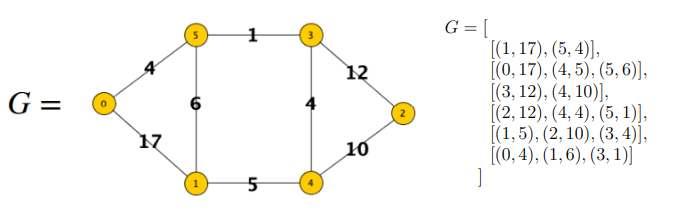
\includegraphics[width=0.8\linewidth]{images/grafi-pesati.PNG}
    \caption{Rappresentazione di grafi pesati}
    \label{fig:grafi-pesati}
\end{figure}

Vedremo ora un algoritmo che permette di trovare i cammini minimi lavorando direttamente su grafi pesati (con pesi anche non interi) l'algoritmo è noto come algoritmo di Dijkstra. 

\subsection{Algoritmo di Dijkstra}
\begin{Algoritmo}{Algoritmo di Dijkstra}{}
    \textit{Dato un grafo pesato vogliamo trovare i cammini minimi e quindi anche le distanze da un certo nodo s (detto sorgente) a tutti gli altri nodi del grafo.} 
    
    Si seguono questi passi:
    \begin{itemize}
        \item costruisci l'albero dei cammini minimi un arco per volta partendo dal nodo sorgente;
        \item ad ogni passo aggiungi all'albero l'arco che produce il nuovo cammino più economico;
        \item alla nuova destinazione assegna come distanza il costo del cammino.
    \end{itemize}

    Un vettore binario \verb|Inserito[x]| ci dice se $x$ è già nell'albero o meno. In \verb|Lista[x]| è presente la coppia $(distanza\_minima, padre)$ il cui significato è il seguente:
    \begin{enumerate}
        \item se $x$ è inserito nell'albero: $padre$ è il suo nodo padre e $distanza\_minima$ la sua vera distanza dalla sorgente;
        \item se $x$ non è inserito nell'albero e non è adiacente ad un nodo inserito nell'albero allora $(distanza\_minima, padre) = (\infty , -1)$;
        \item se $x$ non è inserito nell'albero ma è adiacente a nodi dell'albero allora $padre$ è il nodo dell'albero più conveniente a cui attaccare $x$ e $distanza$ è la distanza minima che ne risulterebbe.
    \end{enumerate}

    All'inizio l'unico nodo nell'albero è la sorgente. Nel seguito i nodi verranno inseriti via via nell'albero e si terminerà solo quando non ci saranno più nodi da inserire o tutti i nodi non ancora inseriti avranno valore $+\infty$ (il che significa che non sono nella stessa componente della sorgente $s$.

    \begin{lstlisting}[language=Python]
    def dijkstra(s, G):
        Inserito=[False]*len(G)
        form math import inf
        Lista=[(inf, -1)]*len(G)
        Lista[s],Inserito[s]=(0, s),True
        for y, costo in G[s]:
            Lista[y]=(costo, s)
        while True:
            minimo=inf
            for i in range(len(Lista)):
                if not Inserito[i] and Lista[i][0]<minimo:
                    minimo,x=Lista[i][0],i
            if minimo==inf:
                break
            Inserito[x]=True
            for y, costo in G[x]:
                if not Inserito[y] and minimo+costo<Lista[y][0]:
                    Lista[y]=(minimo+costo, x)
        D=[costo for costo, _ in Lista]
        P=[padre for _, padre in Lista]
        return D, P
    \end{lstlisting}

    Il costo totale dell'esecuzione delle istruzioni al di fuori del while è $\Theta(n)$. Abbiamo poi un while che viene eseguito al più $n-1$ volte visto che ad ogni iterazione un nodo non inserito viene inserito nell’albero. All’interno del while c’è un primo for che viene iterato ogni volta esattamente $n$ volte ed un secondo for che viene eseguito tante volte quanti sono gli adiacenti presenti nella lista del nodo appena inserito nell’albero (quindi il numero di queste iterazioni è $O(n)$). In pratica ognuna delle $O(n)$ iterazioni del while costa $\Theta(n)$ e quindi il costo del while è $O(n^2)$. La complessità di questa implementazione è dunque $\Theta(n)+O(n^2)=O(n^2)$. Questa implementazione è ottima nel caso di grafi densi dove $m = \Theta(n^2)$.
\end{Algoritmo}

\begin{figure}[ht]
    \centering
    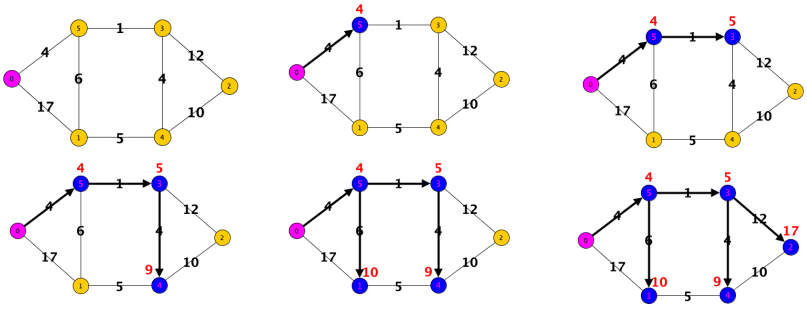
\includegraphics[width=0.8\linewidth]{images/dijkstra.PNG}
    \caption{Esempio algoritmo di Dijkstra}
    \label{fig:dijkstra}
\end{figure}

\begin{Thm}{Correttezza algoritmo di Dijkstra}{}
    La prima cosa da notare è che l'algoritmo non è corretto nel caso di grafi con pesi anche negativi.
    Nel caso di pesi positivi, ad ogni iterazione del while viene assegnata una nuova distanza ad un nodo. Per induzione sul numero di iterazioni mostreremo che la distanza assegnata è quella minima.

    Il caso base è banale (al passo 0 viene assegnata distanza zero alla sorgente e con pesi positivi non può esserci una distanza inferiore). Sia $T_i$ l'albero dei cammini minimi costruito fino al passo $i > 0$ e $(u, v)$ l'arco aggiunto all'albero al passo $i+ 1$. Faremo vedere che $D[v]$ è la distanza minima di $v$ da $s$. Basterà mostrare che il costo di un eventuale cammino alternativo è sempre superiore o uguale a $D[v]$.
    \begin{itemize}
        \item Sia $C$ un qualsiasi cammino da $s$ a $v$ alternativo a quello presente nell'albero e $(x, y)$ il primo arco che incontriamo percorrendo il cammino $C$ all'indietro tale che $x$ è nell'albero $T_i$ e $y$ no (tale arco deve esistere perché $s$ è in $T_i$ mentre $v$ no).
        \item Per ipotesi induttiva $costo(C)\geq Dist(x)+peso(x, y)$ (quest'affermazione è vera perché i pesi del grafo sono tutti non negativi).
        \item L'algoritmo ha preferito estendere l'albero $T_i$ con l'arco $(u, v)$ anziché l'arco $(x, y)$ e in base alla regola con cui l'algoritmo sceglie l'arco con cui estendere l'albero deve quindi aversi $D[x] + p(x, y) \geq D[u] + p(u, v)$. Da cui segue: $costo(C) \geq D[x] + peso(x, y) \geq D[u] + p(u, v) = D[v]$ e il cammino alternativo ha un costo superiore a $D[v]$.
    \end{itemize}
\end{Thm}

Se si potesse evitare di scorrere ogni volta il vettore \verb|Lista| alla ricerca della posizione in cui è presente il minimo potrei evitare di pagare $\Theta(n)$ ad ogni iterazione del while. 

\begin{Algoritmo}{Algoritmo di Dijkstra con heap minimo}{}
     Per ogni nodo $x$ del grafo per cui c'è arco $(p, x)$ con $p$ nell'albero e $x$ non nell’albero, posso mantenere in un heap minimo la tripla $(D[p]+costo(p, x), x, p)$ (indicizzata rispetto alla prima componente). In questo modo ad ogni step possiamo scoprire in tempo logaritmico nella dimensione dell'heap il nodo $x$ da inserire nell'albero, il costo $D[p]+costo(p, x)$ da assegnargli e il padre $p$ a cui agganciarlo. Ovviamente ogni volta che aggiungo un nodo all'albero dovrò aggiornare anche l'heap inserendovi nuovi valori $(D[x]+costo(x, y), y, x)$ per ogni vicino $y$ di $x$ (ricorda che ogni
inserimento ha costo logaritmico nella dimensione dell'heap).

    \begin{lstlisting}[language=Python]
    def dijkstra(s, G):
        P=[-1]*len(G)
        from math import inf
        D=[inf]*len(G)
        D[s], P[s]=0, s
        from heapq import heappop, heappush
        H=[]
        for y, costo in G[s]:
            heappush(H, (costo, s, y))
        while H:
            costo, padre, x=heappop(H)
            if P[x]==-1:
                P[x]=padre
                D[x]=costo
                for y, costo1 in G[x]:
                    heappush(H, (D[x]+costo1, x, y))
        return D, P
    \end{lstlisting}

    Nota che in $H$ possono esserci anche $O(m)$ elementi e quindi i costi di inserimento ed estrazione saranno $O(\log m) = O(\log n^2) = O(\log n)$.
    
    Prima dell’accesso al while abbiamo l’inizializzazione di $D$ e $P$ (per un costo $O(n)$) e l’inserimento nell’heap $H$ di $O(n)$ elementi (per un costo $O(n \log n)$). Abbiamo un while con all’interno un for.
    Ad ogni iterazione del while si elimina un elemento da $H$ e eventualmente per mezzo del for annidato si scorre la lista di adiacenza di un nodo e vengono aggiunti elementi ad $H$. Ogni lista di adiacenza può essere scorsa al più una volta quindi ad $H$ in totale possono essere aggiunti al più $O(m)$ elementi. Per quanto detto il numero di iterazioni del while è $O(m)$. Il costo di ciascuna iterazione del while richiede $O(\log n)$ a causa dell’estrazione da $H$. Quindi il costo totale del while, senza tener conto del for, sarà $O(m \log m)$. Il tempo totale richiesto dalle varie iterazioni del for annidato nel while è $O(m \log n)$ in quando ad ogni iterazione scorro una lista di adiacenza diversa. In totale scorrerò $O(m)$ archi e per ogni arco pagherò $O(\log n)$ per inserimento in $H$. La complessità di questa implementazione è dunque $O(n \log n) + O(m \log n) + O(m \log n) = O((n + m) \log n)$.

    Questa soluzione nel caso di grafi sparsi ha una complessità $O(n \log n)$, mentre andrebbe evitata nel caso di grafi densi dove la complessità risultante sarebbe $O(n^2 \log n)$.
\end{Algoritmo}

\subsection{Minimo albero di copertura}
In alcuni problemi è richiesta la ricerca nel grafo di un albero che “copre” l’intero grafo e la cui somma dei costi dei suoi archi sia minima. Questo problema prende il nome di \textit{minimo albero di copertura}.

\begin{Algoritmo}{Algoritmo di Kruskal}{}
    \textit{Dato un grafo $G$ connesso e pesato cerchiamo un suo minimo albero di copertura.}

    L'algoritmo opera come segue:
    \begin{itemize}
        \item Parti con il grafo $T$ che contiene tutti i nodi di $G$ e nessun arco di $G$.
        \item Considera uno dopo l’altro gli archi del grafo $G$ in ordine di costo crescente.
        \item Se l’arco forma un ciclo in $T$ con archi già presi allora non prenderlo altrimenti inseriscilo in $T$.
        \item Al termine restituisci $T$.
    \end{itemize}

    Quindi con un pre-processing ordino gli archi in $E$ in ordine decrescente cosicché l'estrazione da $E$ dell'arco di costo minimo costi $O(1)$. Verifico che l’arco $(x, y)$ non formi un ciclo in $T$ controllando se $y$ è raggiungibile da $x$ in $T$.

    \begin{lstlisting}[language=Python]
    def kruskal(G):
        E=[(c, u, v) for u in range(len(G)) for v, c in G[u] if u<v]
        E.sort(reverse=True)
        T=[[] for _ in G]
        while E:
            c, x, y = E.pop()
            if not connessi(x, y, T):
                T[x].append(y)
                T[y].append(x)
        return T

    def connessi(x, y, T):
        def connessiR(a, b, T):
            visitati[a]=1
            for z in T[a]:
                if z==b:
                    return True
                if not visitati[z] and connessiR(z, b, T):
                    return True
            return False

        visitati=[0]*len(T)
        return connessiR(x, y, T)
    \end{lstlisting}

    L'ordinamento esterno al while costa $O(m \log m) = O(m \log n)$, il while viene iterato $m$ volte (non ad ogni passo viene inserito un arco in $T$). L'estrazione dell'arco $(a, b)$ di costo minimo da $E$ richiede tempo $O(1)$, controllare che l'arco $(a, b)$ non crei ciclo in $T$ con la procedura \verb|connessi(a, b, T)| richiede il costo di una visita di un grafo aciclico quindi $O(n)$.

    La complessità di questa implementazione è $O(mn)$.
\end{Algoritmo}

\begin{figure}[ht]
    \centering
    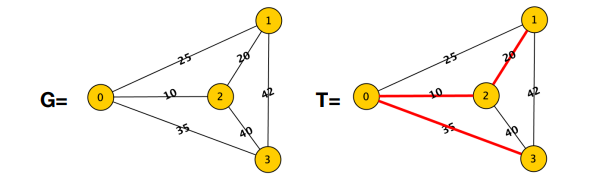
\includegraphics[width=0.7\linewidth]{images/kruskal.PNG}
    \caption{Esempio algoritmo di Kruskal}
    \label{fig:kruskal}
\end{figure}

\begin{Thm}{Correttezza dell'algoritmo di Kruskal}{}
    Dobbiamo far vedere che al termine dell’algoritmo $T$ è un albero di copertura e che non c’è un altro albero che costa meno.

    \begin{demonstration}\phantom{}
    \begin{itemize}
        \item \textit{L'algoritmo produce un albero di copertura}: la prova viene fornita per assurdo. Supponiamo che al termine in $T$ ci sia più di una componente. Consideriamone una $A$, poiché $G$ è connesso nel grafo c’è un arco $(x, y)$ da un nodo $x$ di $A$ ad un nodo $y$ di un’altra componente $B$ ma l’arco $(x, y)$ ad un certo punto è stato estratto da $E$ e se non crea ciclo in $T$ ora che l’algoritmo è terminato non lo creava neanche al momento in cui è stato estratto e quindi sarebbe stato aggiunto a $T$ e non scartato.
        \item \textit{Non c'è un albero di copertura per $G$ che costa meno di $T$}: la prova viene fornita per assurdo. Tra tutti gli alberi di copertura di costo minimo per $G$ prendiamo quello che differisce nel minor numero di archi da $T$. Sia $T^*$. Supponiamo per assurdo che $T$ differisca da $T^*$. Faremo vedere che questa assunzione porterebbe all'assurdo perché avrebbe come conseguenza l'esistenza di un altro albero di copertura di costo minimo per $G$ che differisce da $T$ in meno archi di $T^*$. 
        
        Considera l'ordine $e_1, e_2,...$ con cui gli archi sono stati presi in considerazione nel corso dell'algoritmo e sia $e$ il primo arco preso che non compare in $T^*$. Se inserisco $e$ in $T^*$ si forma di certo un ciclo $C$. Il ciclo $C$ contiene almeno un arco $e'$ che non appartiene a $T$ (infatti non tutti gli archi del ciclo $C$ sono in $T$ altrimenti e non sarebbe stato preso dall'algoritmo di Kruskal). Considera ora l'albero $T'$ che ottengo da $T^*$ inserendo l'arco $e$ ed eliminando $e'$. Il costo del nuovo albero $T'$ (che è $costo(T^*)-costo(e') + costo(e)$) non può aumentare rispetto a quello di $T^*$ (perché $costo(e)\leq costo(e')$, nota infatti che tra i due archi $e$ ed $e'$ che non creavano ciclo Kruskal ha considerato prima l'arco $e$) ma allora $T$ è un altro albero di copertura ottimo che differisce da $T$ in meno archi di quanto faccia di $T^*$ il che contraddice l'ipotesi che $T^*$ differisce da $T$ nel minor numero di archi.
    \end{itemize}
    \end{demonstration}
\end{Thm}

\begin{Algoritmo}{Algoritmo di Kruskal con Union e Find}{}
    Per migliore l'implementazione non possiamo permetterci di spendere $O(n)$ ad ogni iterazione del while a causa della visita per testare la raggiungibilità. Ricorreremo alla struttura dati Union e Find che permette di testare efficientemente se due nodi appartengano o meno alla stessa componente connessa.

    \begin{lstlisting}[language=Python]
    def kruskal(G):
        E=[(c, u, v) for u in range(len(G)) for v, c in G[u] if u<v]
        E.sort(reverse=True)
        T=[[] for _ in G]
        C=crea(T)
        while E!=[]:
            c, x, y = E.pop()
            cx = find(x, C)
            cy = find(y, C)
            if cx!=cy:
                T[x].append(y)
                T[y].append(x)
                union(cx, cy, C)
        return T
    \end{lstlisting}

    L’ordinamento costa $O(m \log n)$, il while viene iterato $m$ volte (non ad ogni passo viene inserito un arco in $T$). L’estrazione dell’arco $(a, b)$ di costo minimo da $E$ richiede $\Theta(1)$, eseguire il Find costa $O(\log n)$, eseguire l’Union costa $\Theta(1)$ (e all’interno del while viene eseguito esattamente $n-1$ volte).
    
    La complessità di questa implementazione è $O(m \log n)$.
\end{Algoritmo}


\section{Union-Find}
L'\textit{Union-Find}, noto anche come Disjoint Set Union (DSU), è una struttura utilizzata per operazioni di unione e ricerca efficienti su insiemi disgiunti. Le tre operazioni fondamentali di Union-Find sono:
\begin{enumerate}
    \item \verb|Crea(S)|: restituisce una struttura dati Union-Find sull’insieme $S$ di elementi dove ciascun elemento è in un insieme separato. 
    \item \verb|Find(x, C)|: Restituisce il nome dell'insieme della struttura dati $C$ a cui appartiene l’elemento $x$.
    \item \verb|Union(A, B, C)|: modifica la struttura dati $C$ fondendo i due suoi insiemi di nome $A$ e $B$ in un singolo insieme.
\end{enumerate}

Una gestione efficiente di insiemi disgiunti è utile in diversi contesti. 

\begin{Example}{Union-Find con grafi}{}
    \textit{Si pensi ad esempio allo scenario dove un grafo evolve nel tempo con l’aggiunta di archi.} 
    
    In questo caso gli insiemi disgiunti sono le componenti connesse del grafo. L’operazione \verb|find(u)| sul nodo $u$ permette di scoprire in quale componente si trova il nodo $u$. L’operazione può essere usata per testare se due nodi $u$ e $v$ sono nello stessa componente semplicemente verificando se \verb|find(u)==find(v)|.

    Se poi l’arco $(u,v)$ viene aggiunto al grafo allora prima si testa se $u$ e $v$ sono nella stessa componente connessa e se risulta $A\neq B$ dove \verb|A=find(u)| e \verb|B=find(v)| l’operazione \verb|Union(A, B)| può essere usata per fondere le due componenti.
\end{Example}

Come primo approccio possiamo pensare di assegnare all’insieme il nome dell’elemento massimo in esso contenuto.

\begin{Algoritmo}{Union-Find}{}
    Probabilmente il modo più semplice di implementare questa struttura dati per $n$ elementi è di mantenere il vettore $C$ delle $n$ componenti. All’inizio ogni elemento è in un insieme distinto vale a dire $C[i]=i$. Quando la componente $i$ viene fusa con la componente $j$, se $i>j$ allora tutte le occorrenze di $j$ nel vettore $C$ verranno sostituite da $i$ (se $i<j$ accadrà il contrario).

    \begin{lstlisting}[language=Python]
    def Crea(G):
        C=[i for i in range(len(G))]
        return C

    def Find(u, C):
        return C[u]

    def Union(a, b, C):
        if a>b:
            for i in range(len(C)):
                if C[i]==b:
                    C[i]=a
        else:
            for i in range(len(C)):
                if C[i]==a:
                    C[i]=b
    \end{lstlisting}

    Il costo delle operazioni è rispettivamente $\Theta(n)$, $\Theta(1)$, $\Theta(n)$.
\end{Algoritmo}

Nella implementazione appena vista al \verb|Find| costa $O(1)$ e la \verb|Union| $\Theta(n)$. Meglio bilanciare i costi utilizzando il vettore dei padri.

\begin{Algoritmo}{Union-Find con il vettore dei padri}{}
    In questa implementazione quando voglio sapere in che componente si trova un nodo devo semplicemente risalire alla sua radice in tempo $O(n)$, mentre quando fondo due componenti una diventa figlia dell'altra in $O(1)$.

    \begin{lstlisting}[language=Python]
    def Crea(G):
        C=[i for i in range(len(G))]
        return C

    def Find(u, C):
        while u!=C[u]:
            u=C[u]
        return u

    def Union(a, b, C):
        if a>b:
            C[b]=a
        else:
            C[a]=b
    \end{lstlisting}
\end{Algoritmo}

Se non voglio arrivare a spendere $O(n)$ per la \verb|Find| i cammini per arrivare alle radice del vettore dei padri non devono essere mai troppo lunghi. Dunque è meglio mantenere gli alberi bilanciati.

Quando con la \verb|Union| fondo le due componenti rendo sempre radice la componente che ha più elementi. L'intuizione è che in questo modo per almeno la metà dei nodi presenti nelle due componenti  coinvolte nella fusione la lunghezza del cammino non aumenta. 

\begin{Algoritmo}{Union-Find con alberi bilanciati}{}
    In questa implementazione della Union-Find devo fare in modo che ai nodi radice sia associato anche il numero di elementi che la componente contiene. 
    Ogni elemento è caratterizzato da una coppia $(x, numero)$ dove $x$ è il nome dell’elemento e $numero$ è il numero di nodi nell’albero radicato in $x$.

    \begin{lstlisting}[language=Python]
    def Crea(G):
        C=[(i, 1) for i in range(len(G))]
        return C

    def Find(u, C):
        while u!=C[u]:
            u=C[u]
        return u

    def Union(a, b, C):
        tota, totb = C[a][1], C[b][1]
        if tota>=totb:
            C[a]=(a, tota+totb)
            C[b]=(a, totb)
        else:
            C[b]=(b, tota+totb)
            C[a]=(b, tota)
    \end{lstlisting}
\end{Algoritmo}

Con questo accorgimento nella fusione delle componenti vale la seguente proprietà: se una componente ha altezza $h$ allora la componente contiene almeno $2^h$ nodi. Dalla proprietà deduciamo che l’altezza delle componenti non potrà mai superare $\log n$ (perché in caso contrario avrei nella componente più di $n$ nodi il che è assurdo). Implementando quindi nella \verb|Union| l’accorgimento descritto la \verb|Find| richiederà tempo $O(\log n)$ anziché $O(n)$.

\begin{Lemma}{Proprietà degli alberi bilanciati}{}
    \textit{Se una componente ha altezza $h$ allora la componente contiene almeno $2^h$ nodi.}

    \begin{demonstration}
        Assumiamo per assurdo durante una delle fusioni si sia formata un nuova componente di altezza $h$ che non rispetta la proprietà. Considera la prima volta che ciò accade e siano $ca$ e $cb$ le componenti che si fondono. Possono essere accadute due cose:
        \begin{itemize}
            \item $ca$ e $cb$ erano componenti con la stessa altezza allora avevano entrambe altezza $h-1$ ed ognuna aveva almeno $2^{h-1}$ elementi (perché nelle fusioni precedenti la proprietà era sempre stata verificata). Quindi il numero totale di elementi della nuova componente è $2^{h-1}+2^{h-1}=2^h$ e la proprietà è verificata.
            \item $ca$ e $cb$ avevano diverse altezze allora l’altezza dopo la fusione è quella della componente di altezza maggiore che doveva essere già altezza $h$ e conteneva da sola già $2^h$ elementi.
        \end{itemize}
    \end{demonstration}
\end{Lemma}